In this section, we evaluate our methods on classification tasks with both synthesized data and real world data.

\subsection{Experiment setup}

We compare both of our algorithms: \textbf{Adaptive Difficulty EM} and \textbf{Fixed Difficulty EM} with two baselines: \textbf{Majority Voting} and \textbf{Original EM} \cite{raykar2010learning}.   We compare their performance mainly in three aspects: 
\begin{itemize}
    \item How well they can estimate the ground truth
    \item The generalization of the learnt classifier
    \item How well they can estimate the expertise of each expert, i.e. sensitivity and specificity.
\end{itemize}

% 感觉这段还能改,语言上有点不清晰,不过先不动
%你改改,我先睡睡

For synthesized data, we sample 2000 two-dimensional data points from a two-class Gaussian mixture with a known Bayesian classification boundary.

%We use a synthesized two-dimensional dataset and a image dataset in our experiments. The two-dimensional dataset is a two-class Gaussian mixture containing 2000 datapoints.

For the real data, we tried to collect real crowdsourced labels, but it's  difficult and expensive to obtain real crowdsourced labels. We use the \textbf{Dogs vs. Cats} \citep{kaggle2013} dataset, which consists of $25,000$ images from $2$ classes, dogs and cats and their golden ground truth label.

Note for the above two data set, the real crowdsourced labels are inaccessible, we use the ground truth label to simulate crowdsourced label in two ways: firstly, we simulate noisy labels with pre-chosen confusion matrix, where the labels are more structural, and coincide to our assumption ; secondly, the probability of worker making wrong decision is sampled from a certain discrete distribution, where the labels are more non-structural.
%first, totally under our the assumption of our algorithm; second, nearly not obeying our assumption. % 我这一句没说好,就是不符合我们的生成假设,怎么用英文说2333
%do not matchooko???? I do not understand ?? use wechat pls

For the rest of this section, we organize our text as below:
We cover the details of the synthesized data set in subsection \ref{4.2}, and analyze the performance of each algorithm on this data in subsection 4.3;  In subsection 4.3 we cover the performance analysis of the \textbf{Dogs vs. Cats} dataset, on both structural (4.3.1) and non-structural (4.3.2) labels.

\subsection{Two-dimensional Gaussian Mixture dataset}\label{4.2}

To validate our methods, we use two-dimensional Gaussian mixture with a known Bayesian classification boundary in order to explicitly incorporate the difficulty of datapoint, i.e. the distance to the decision boundary.

In our experiments, we synthesize a Bayesian classification boundary($x+y=0$) and two Gaussians(mean= (1,1),variance= 1 \& mean= (-1,-1),variance= 1). The Gaussian dataset contains 1000 training datapoints and 1000 test datapoints. The classification method used here is logistic regression. We use the distance of each  datapoint to the Bayesian classification boundary to the difficulty of each datapoint.

As for the labels, we use five experts with sensitivity $\alpha$ = [0.8 0.6 0.6 0.7 0.6] and specificity $\beta$ = [0.6 0.7 0.6 0.7 0.7] to determine the the sensitivity ability $\bm{\lambda^1}$ and the specificity ability $\bm{\lambda^2}$ of experts. We used both the sensitivity and specificity of experts and datapoint difficulty to recover the parameters of experts at every specific datapoint to synthesize the crowdsourced labels (refer to equation (1) and (2)). For concision, we defer the experiment details to the Appendix.

Based on the labels from multiple experts, we can simultaneously:\\ \textbf{(1)} estimate the golden ground truth, \textbf{(2)} learn a logistic-regression classifier, and \textbf{(3)} estimate the sensitivity and specificity of each expert.

So we compare on three different aspects:
    \textbf{(1)} How good is the estimated ground truth?
    \textbf{(2)} How good is generalization of the learnt classifier?
    \textbf{(3)} How well can we estimate the sensitivity and specificity of each expert?


\subsubsection{Results}


\textbf{1. Estimated ground truth}

Since the estimates of the actual ground truth are probabilistic scores, we can plot the \textbf{ROC curves} of the estimated ground truth. Note the in all EM-based algorithms, we use the output of the converged value in E step (i.e. $\textup{Pr}[y_i=1|y_i^1,...,y_i^R,\bm{x_i},\bm{\theta} ]$) as the estimated probability. From Figure \ref{fig:gr} we can see that the ROC curve for the proposed methods are superior to the majority voting and the original EM algorithm. The proposed algorithm appropriately weights each expert based on their estimated parameters $\bm{\lambda}$. The average expertise of expert is low so the learning process with majority voting labels is highly biased. 

\begin{figure}[htbp]
    \centering
    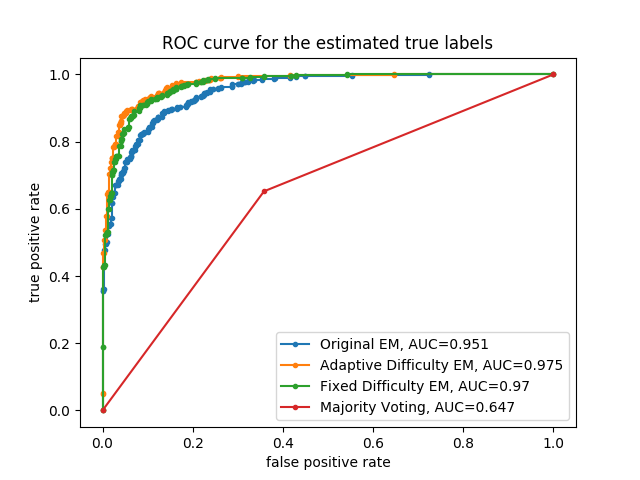
\includegraphics[width=5.0in]{image/roc_plot.png}
    \caption{ROC Curve for the estimated true labels. We compare our proposed methods with \textbf{Majority Voting} and \textbf{Original EM}} 
    \label{fig:gr}
\end{figure}

\textbf{2. Generalization of the learnt classifier}

From Table \ref{table:gt} we can see the generalization property of the learnt classifier is consistently well in all EM-based algorithms. Surprisingly, the proposed \textbf{Fixed Difficulty EM} algorithm increases the accuracy by a large margin but the AUC of it on the training set is inferior to \textbf{Adaptive Difficulty EM}. Our hypothesis is that the fixed imaged difficulty can play the role of regularization.

\begin{table}[H]
\caption{Guassian dataset: Accuracy of learnt classifier on test set}
\label{table:gt}
\begin{center}
\begin{tabular}{c c c c c }
		\toprule
		Method & Majority Voting & Original EM & Adaptive Difficulty EM & Fixed Difficulty EM	 \\
		\midrule
        Accuracy & $93.6 \pm 0.05$  & $94.00 \pm 0.11$ & $93.9 \pm 0.15$ & $\bm{94.4 \pm 0.13}$ \\
		\bottomrule
\end{tabular}
\end{center}
\end{table}

\textbf{3. Estimated expertise}

The actual sensitivity and specificity of each expert is marked as blue dots in Figure \ref{fig:ge}. We can see that the estimated expertise of our proposed EM algorithms is much closer to the actual values of sensitivity and specificity than the original EM algorithm. Moreover, we find that the estimated expertise of the two proposed algorithm is close. So different interpretations of image difficulty do not change the updating trajectory of experts' parameters much. We use $\alpha = \sigma (\frac{\bm{\lambda}^{1}}{4})$ and $\beta = \sigma(\frac{\bm{\lambda}^{2}}{4})$to recover the sensitivity and specificity of experts.

\begin{figure}[H]
    \centering
    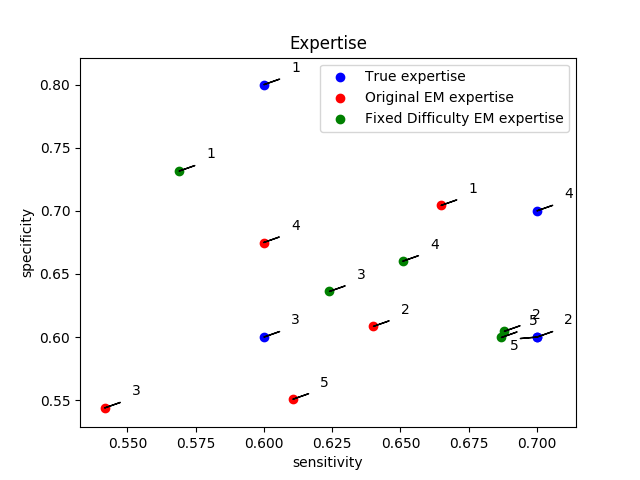
\includegraphics[width=5in]{image/expertise_g.png}
    \caption{Estimated Expertise on Gaussian dataset. The numbers denote corresponding experts. The expertise of \textbf{Adaptive Difficulty EM} and \textbf{Fixed Difficulty EM} is very close, so we only plot one of them. } 
    \label{fig:ge}
\end{figure}


\subsection{Dogs vs. Cats dataset}

In this experiments, the expert label real-world 2-class dataset. The experiment set up is almost the same as the two-dimension Gaussian mixture dataset except that the classifier used in this experiment is a four-layer convolutional neural network, and we use a pre-trained four-layer convolutional neural network to synthesis image difficulty, i.e the more uncertain the pretrained classifier is the more difficult this data point is.
We manually split the dataset into a $12,500$-image training set and a $12,500$-image test set to both test the accuracy of the estimated ground truth on the training set and the generalization performance of the learnt classifier on the test set.

\subsubsection{Structural Label}
Table \ref{table:dt}, Figure \ref{fig:dr} and Figure \ref{fig:de} summarize the results. The proposed \textbf{Fixed Difficulty EM} algorithm performs well both on estimating true labels and the generalization. The estimated expertise of \textbf{Original EM} marginally closer to the ground-truth expertise. 

We can see that \textbf{Majority Voting} can not converge in this case, and \textbf{Original EM} converges poorly. Actually, \textbf{Original EM} even can not converge in some experiments.


\begin{table}[htp]
\caption{Dogs vs. Cats dataset: Accuracy of learnt classifier on test set}
\label{table:dt}
\begin{center}
\begin{tabular}{c c c c c }
		\toprule
		Method & Majority Voting & Original EM & Adaptive Difficulty EM & Fixed Difficulty EM	 \\
		\midrule
        Accuracy & $50.0 \pm 0.0$  & $60.2 \pm 9.1$ & $70.4 \pm 0.9$ & $\bm{74.3 \pm 1.7}$ \\
		\bottomrule
\end{tabular}
\end{center}
\end{table}

\begin{figure}[htb]
    \centering
    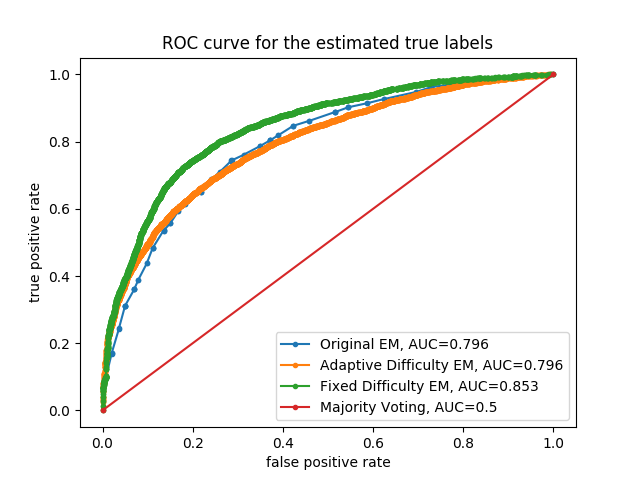
\includegraphics[width=5.5in]{image/roc_plot_dog.png}
    \caption{ROC Curve for the estimated true labels. We compare our proposed methods with \textbf{Majority Voting} and \textbf{Original EM}} 
    \label{fig:dr}
\end{figure}

\begin{figure}[htb]
    \centering
    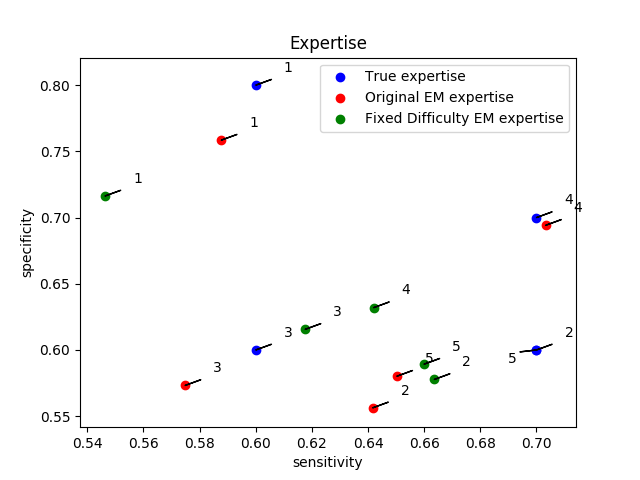
\includegraphics[width=5.5in]{image/expertise_dog.png}
    \caption{Estimated Expertise on Dogs vs Cats dataset. The numbers denote corresponding experts. The expertise of \textbf{Adaptive Difficulty EM} and \textbf{Fixed Difficulty EM} is very close, so we only plot one of them. } 
    \label{fig:de}
\end{figure}

\subsubsection{Non-structural Label}
Since in the experiments above, we use our assumption to synthesize the experts' labels, which is very structural. So we would like to compare these methods under settings that may be closer to real world, where the labels tend to be less structural. In such settings, with regard to every datapoint, an expert makes mistakes with probability $\frac{1}{3+k}$, where k is uniformly sampled from $\{0,1,2,3,4,5\}$. It should be noted that, to a single expert, the error probabilities corresponding to different images are also different. We only compare the generalization ability of the learnt classifier. The result is shown in Table \ref{table:rt}. The proposed algorithms still dominate other algorithms in this setting. The other two algorithms can not converge using non-structural labels.

\begin{table}[htp]
\caption{Non-structural label: Accuracy of learnt classifier on test set}
\label{table:rt}
\begin{center}
\begin{tabular}{c c c c c }
		\toprule
		Method & Majority Voting & Original EM & Adaptive Difficulty EM & Fixed Difficulty EM	 \\
		\midrule
        Accuracy & $50.0 \pm 0.0$  & $50.6 \pm 0.6$ & $76.7 \pm 0.8$ & $\bm{78.2 \pm 0.3}$ \\
		\bottomrule
\end{tabular}
\end{center}
\end{table}